\section{Convolutional Networks}
\subsection{Convolution}
\textbf{Integral Operators: }$(Tf)(u) = \int_{t_1}^{t_2} G(u,t)f(t) dt$ with a kernel $G: \mathbb{R}^2 \rightarrow \mathbb{R}$
\textbf{Convolution: }$(f * g)(u) := \int_{-\infty}^{\infty} g(u-t)f(t) dt = \int_{-\infty}^{\infty} f(u-t)g(t) dt = (g*f)(u)$ integral operator with kernel $G(u,t) = g(u-t)$\\
\textbf{Shift equivariance: }Let $f_{\Delta}(t) = f(t + \Delta)$ be a shifted fct. Convolution is shift-equivariant: $\forall \Delta \in \mathbb{R}: f_{\Delta}*g = (f*g)_{\Delta}$ because of the shift invariance of the kernel: $G(u-\Delta, t-\Delta) = g(u-t) = G(u,t)$  $\forall \Delta$\\
\textbf{Any translation equivariant operator is a convolution}
\textbf{Fourier transform:} $\mathcal{F}(f)(u) := \int_{-\infty}^{\infty} e^{-2\pi itu} f(t) dt$\\
Convolutional operators can be computed via pointwise multiplications in Fourier space: $\mathcal{F}(f*g) = \mathcal{F}(f) \cdot \mathcal{F}(g)$ and the \textbf{Inverse Fourier transform} maps it back to the input space $f*g = \mathcal{F}^{-1}((\mathcal{F}(f) \cdot \mathcal{F}(g)))$. Computations of convolutions: Naive $\mathbf{O}(n^2)$, FFT $\mathbf{O}(n \log n)$\\
\textbf{Linear shift equivariant transforms:} A convolution can also be characterized as a linear shift invariant operator (1)$T(\alpha f + \beta g) = \alpha Tf + \beta T g$, (2) $(Tf_{\Delta})(t) = (Tf)(t+\Delta)$. \textcolor{violet}{Any linear, translation equivariant transformation T can be written as a convolution with a suitable kernel.}\\
\textbf{Discrete Convolution: }$(f*g)[u] = \sum_{t = -\infty}^{\infty} f[t]g[u-t]$ \textrightarrow \textit{commutative}\\
\textbf{Cross-correlation: }$(g \star f)[u]:= \sum_{t = -\infty}^{\infty} g[t]f[u+t] = (\Bar{g}*f)[t]$ where $\Bar{g}[t] = g[-t]$ \textrightarrow \textit{non-commutative}\\
\textbf{Toeplitz matrix:} if the f,g have finite support (f[t] = 0 $\forall t \notin [1:n]$, $g[t] = 0$ $\forall t \notin [1:m]$ and $m \leq n$ we have $(f*g) = $
\begin{pmatrix}
g_{1} & 0     & 0     & \cdots & 0     & 0 \\
g_{2} & g_{1} & 0     & \cdots & 0     & 0 \\
\cdot & \cdot & \cdot & \cdots & \cdot & \cdot \\
0      & 0     & 0     & \cdots & g_{m}   & g_{m-1} \\
0      & 0     & 0     & \cdots & 0       & g_{m}

\end{pmatrix}
$\cdot$
\begin{pmatrix}
f_{1}\\
f_{2}\\
\vdots\\
f_{n}
\end{pmatrix}\\
number of free parameters is dim(g) = m
\subsection{Convolutional Networks}
Goal: Define layered arch. for signal processing that exploits translation equivariance, locality and scale => learn kernel fct/filters from data.\\
\textbf{2D discrete convolution: }Extend conv. to higher dimensions by using matrices/tensors.
$(F*G)[i,j] = \sum_{k = -\infty}^{\infty} \sum_{l = -\infty}^{\infty} F[i-k,j-l]G[k,l]$. Convolved signal inherit topology from the original signal so units in a conv layer are usually arranged on the same grid as the input (1d, 2d,..) \\
%\vspace{-1em}
%\begin{center}
%    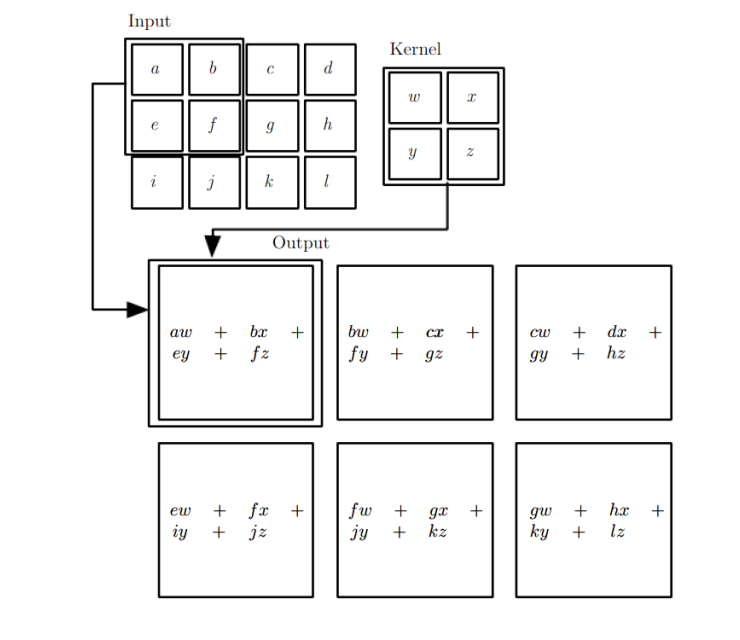
\includegraphics[scale = 0.1]{contents/imgs/conv_kernel.png}
%\end{center}
\textbf{Pooling:} Let $r$ be window size, then $x_{ij}^{\max} = \max \{x_{i+k,j+l} : 0\leq k,l < r\}$ (also avg, min...) is max pooling. Using strides when pooling downsizes. \\
\textbf{Channels:} Learn multiple filters(width) per layer. All channels use the same window size and number of channels is a design parameter. Channels are permutation invariant and connections across channels are dense.
\subsection{Backpropogation of CNN}
\textbf{Receptive Fields:} Receptive field of $x_i^l$: $\mathcal{I}_i^l := \{j: w_{ij} \neq 0\}$ where $W^l$ is the toeplitz matrix of the convolution (includes all the elements in the previous layer that effect the calculation of $x_i^l$). Then $\frac{\partial x_i^l}{\partial x_j^{l-1}} = 0$ for $j\notin \mathcal{I}_i^l$.\\
Con: local receptive field make it hard to connect distant features.\\ 
\textbf{Weight sharing: }When computing the loss gradients $\partial h/\partial g_j^l$ ($g_j^l$ is a kernel weight) we have to respect the weight sharing: $\frac{\partial h}{\partial g_j^l} = \sum_i \frac{\partial h}{\partial x_i^l}\frac{\partial x_i^l}{\partial g_j^l}$. The sum over units appears as the same weight is re-used for every unit within the target layer.
\begin{itemize}
    \item $\nabla_v (v^T \text{vec}(\sigma(x*w))) = \text{vec}(\sigma(x*w)))$
    \item $\nabla_A v^T \text{vec}(A) = mat(v)$
    \item $\nabla_w (x*w) \in \mathbb{R}^{q\times q \times r \times r}$ if $(x*w) \in \mathbb{R}^{r\times r}$, $w \in \mathbb{R}^{q\times q}$
    \item $\nabla_w(v^T \text{vec}(\sigma(x*w))) = \text{rot}_{\pi}(x) * B$ where $B = \text{mat}(v)\odot \sigma'(x*w)$\\
    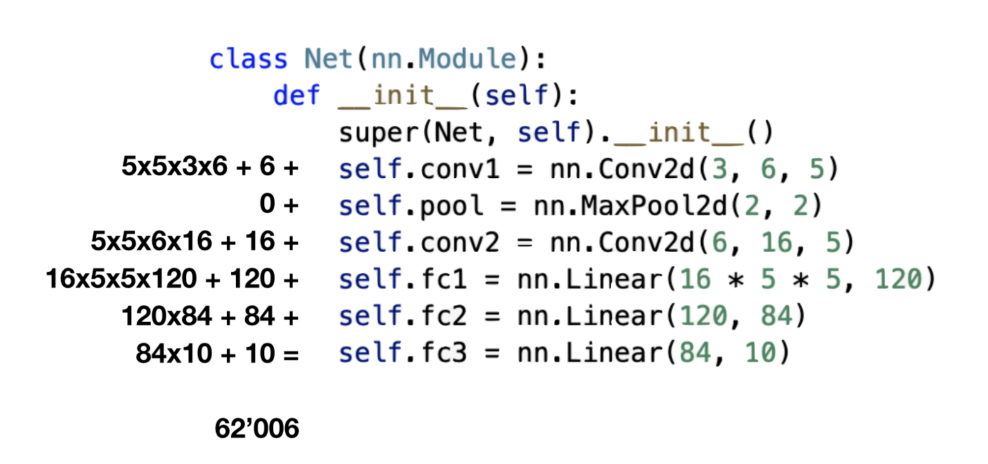
\includegraphics[scale = 0.2]{contents/imgs/n_params_conv.png}
\end{itemize}
%\subsection{Pyramidial Architecture}
%Successful design pattern in computer vision is pyramid like. As you stack convolutions you reduce the spatial resolution of the feature maps with depth while increasing the number of channels. Fina layers are FC.\\
%Important to keep in mind: (1) Avoid blowup of \# parameters to control performance, (2) large Depth is a plus, (3) Allow for a sufficient number of channels  (large width for high accuracy). These 3 things have to be traded off.
%\subsection{VGG}
%Very deep conv. networks. Avoids blowup of the \# parameters and allows for a sufficient number of channels. Uses very small receptive fields (small kernel windows) and avoids downsampling and pooling. Depth is increased to model larger receptive fields.
\subsection{Inception Network}
Deep stacking, uses many channels for accuracy. Dimension reduction in between convolutions (compression of m channels) using a $1\times 1\times m$ convolution with $k\leq m$: $x_{ij}^+ = \sigma(Wx_{ij})$ ; $W \in \mathbb{R}^{k\times m}$
\begin{itemize}
    \item $1\times 1$ part means there is no spatial conv. performed
    \item Not committing to a certain window size, but solve trade-off problem a part of the learning by multiple processing paths
    \item Softmax layers to improve learning dynamics (shortcut error backprop)
\end{itemize}
%\subsection{U-net (image segmentation)}
%\begin{itemize}
%    \item Encoder-Decoder arch.
%    \item Skip connection between encoder and decoder (combine low- and high-level features and local and global features) => solves the problem of long-range correlations.
%\end{itemize}
\subsection{Embeddings}
Enable processing of non-numeric sequences via DNN's by embedding symbols in vector space. $\Omega$ is the alphabet of symbols; $\Omega \ni \omega \mapsto x_{\omega} \in \mathbb{R}^n$. Embedding $\{x_{\omega}\}$ are learnable parameters.\\
\textbf{Word2vec:} Learn input and output embeddings: $\Omega_{in} \ni \omega \mapsto x_{\omega} \in \mathbb{R}^n$ and $\Omega_{out} \ni \nu \mapsto y_{\nu} \in  \mathbb{R}^n$. \\Combine: $\mathbb{P}(\nu|\omega) = \frac{\exp[x^T_{\omega}y_{\nu}]}{\sum_{\mu}\exp[x^T_{\omega}y_{\mu}]}$
and use to predict an output word $\nu$ in neighbourhood of an input word $\omega$

